\section{Introduction}
In recent decades UAV technology is becoming increasingly more accessible as today’s manufacturing enables cheaper, smaller, and more powerful electric motors. Companies such as Drone up\cite{com1}, Wing\cite{com2} and DHL\cite{com3} are developing autonomous drones to enable companies to deliver packages. Other projects such as Europe's \emph{SKYOPENER} \cite{com4} aim to expand civilian applications of Remotely Piloted Aircraft Systems (RPAS).\\
There is some discussion over the efficiency of drones in comparison to electric vehicles. A 2019 study \cite{eff1} found that switching entirely to drones would not be desirable in terms of total efficiency but could be useful in a last-mile approach for light and short distance deliveries. \emph{RAND Corporation}, a research organization,\cite{eff2} estimates that if 20\% of deliveries were replaced by drones this could decrease diesel consumption of the United Parcel Service (UPS) by 5.7\%, reducing the carbon footprint due to trucking as they are converted to electric substitutes.

\vspace{0.5cm}
\begin{wrapfigure}{h}{0.32\textwidth}
\centering
    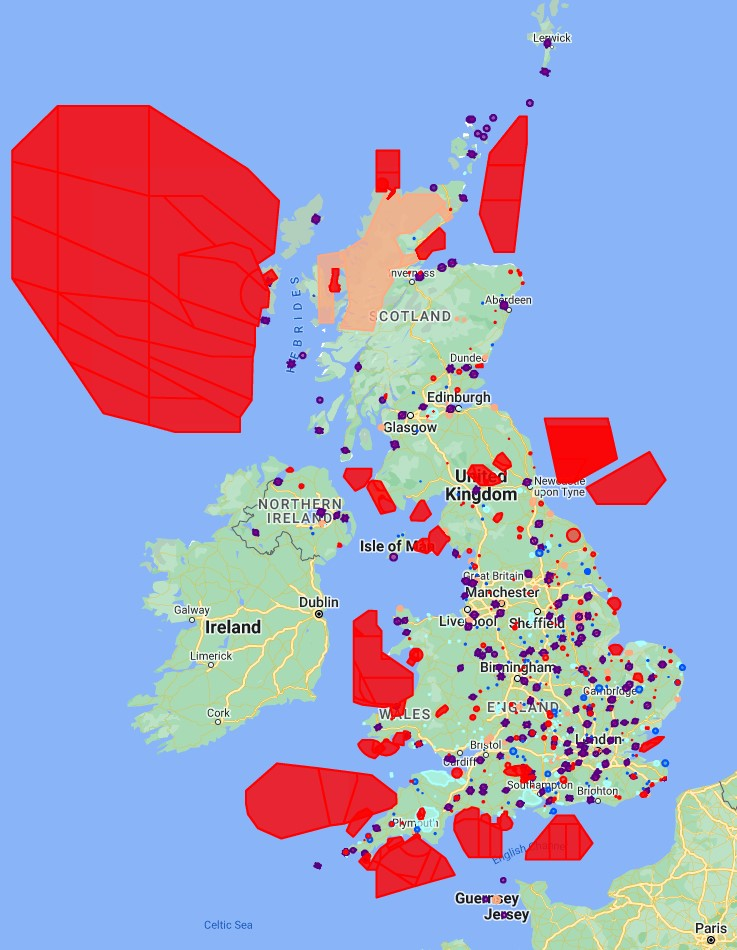
\includegraphics[width=0.3\textwidth]{figures/NoFly.jpg}\hfill
    \caption{UK restricted airspace}
    \label{fig:nofly}
\end{wrapfigure}

Drone flight is already somewhat controlled via legislation, figure \ref{fig:nofly} shows restricted zones in the UK\cite{res1}. One can see how this would become a complex guidance control problem especially if a drone needs to interact with other UAVs, with which it does not have direct communication.   A city council or other similar entity might want more localised control over which airspace is used and when this is the case. As the drone industry expands and evolves so does the control problem. By using reinforcement learning drones might be able to adapt. 

This essay looks at a hypothetical future where drones are used on a much larger scale. Being as easily manoeuvrable as they are and some drones having a range of up to 100km \cite{far1} (although high-end consumer drones manage about 10-15km \cite{far2}) the risk of malicious use of drones is a threat that should not be taken lightly.\cite{ter1} If drones are used more frequently, we may be dependent on the network they provide. Cyber-attacks could be a way of causing havoc and affecting supply chains. For this reason, measures should be prepared to mitigate these risks to the maximum extent. Anti-drone technology is available\cite{ter2} and companies such as D-fend \cite{ter3} are already working towards the solution although a full consensus is yet to be arrived at as different systems each has risks and limitations\cite{ter4}.

While fixed-wing UAVs benefit from flocking in the same way as migratory birds do quad-copter drones do not. Therefore, this application focuses on how to control drone traffic of general UAVs. As it allows for a general agent to be created which can adapt in real-time. If a general agent can be created this could reduce the problem of scaling as all computing could be achieved by individuals.
In this investigation, a reinforcement learning agent will be trained to optimise drone traffic by layering boid flocking behaviour and potential functions. This will mean that multiple agents will come to a general consensus on a trajectory through sensing the aggregate of proximal agent headings and positions.
\clearpage